\section{Chain E -- Link Status Handler, Flush and ThingSpeak}

Maintains an ordered list of outgoing link costs, keyed by
$(\text{ZigBee source}, \text{destination})$ pairs. Rows are appended
in the order Link Status messages are processed; when a pair is seen
again, its cost is updated \emph{in place} so that the row preserves
its original sequence number. Once the 200-message budget is
exhausted, the list is flushed to \texttt{outgoing\_cost.csv} in
processing order, and the smallest source's destinations are then
sorted hexadecimally and streamed to a public ThingSpeak channel at
one update every 20\,s.

\begin{figure}[h]
    \centering
    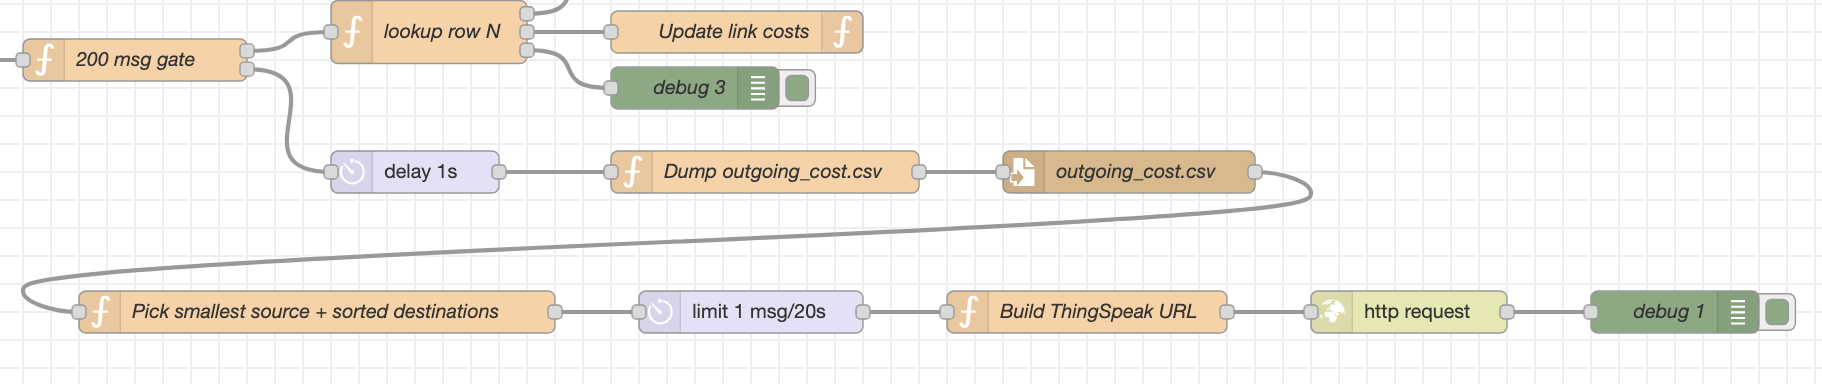
\includegraphics[width=\linewidth]{images/flow_chain_e.png}
    \caption{Chain E -- Link Status update, end-of-run flush and ThingSpeak publisher.}
\end{figure}

\begin{description}
    \item[Function \emph{Update link costs}] (wired to router output~2)
        parses the Command String and iterates the \texttt{Links}
        array. Two data structures are maintained in the global
        context: an ordered \verb|linkRows| array (the rows that will
        ultimately be written to disk, in processing order) and an
        index \verb|linkRowIdx| mapping the key
        \texttt{"src|dst"} to its position in the array. A new
        $(\text{src},\text{dst})$ pair is appended; a repeated pair has
        only its cost updated in place, leaving its row number
        unchanged, as recommended in the clarifications.
        \begin{lstlisting}[]
        const row    = msg.lookup.row;
        const cmdStr = msg.lookup.cmdStr;
        
        const source = String(row["Source Address ZigBee"] || "").trim().toLowerCase();
        if (!source.startsWith("0x")) return null;
        
        let obj;
        try { obj = JSON.parse(cmdStr.replace(/'/g, '"')); }
        catch (e) { node.warn("Link Status parse failed: " + e.message); return null; }
        
        const links = obj.Links;
        if (!Array.isArray(links)) return null;
        
        let rows = global.get('linkRows')   || [];
        let idx  = global.get('linkRowIdx') || {};
        
        for (const link of links) {
            const dest = String(link.Address || "").trim().toLowerCase();
            const cost = parseInt(link["Outgoing Cost"], 10);
            if (!dest.startsWith("0x") || isNaN(cost)) continue;
        
            const key = source + "|" + dest;
            if (idx[key] !== undefined) {
                rows[idx[key]].cost = cost;
            } else {
                idx[key] = rows.length;
                rows.push({ src: source, dst: dest, cost: cost });
            }
        }
        global.set('linkRows', rows);
        global.set('linkRowIdx', idx);
        return null;
        \end{lstlisting}
    \item[Delay (\emph{1\,s})] introduced after the gate's EOF output
        to let the 200th message finish propagating through chain~D
        and the link-cost updater before the flush starts.
    \item[Function \emph{Dump outgoing\_cost.csv}] guarded by a
        single-shot flag, iterates the \verb|linkRows| array in its
        natural (processing) order and emits one CSV row per entry,
        with an incremental \texttt{No.}\ field. No sorting is applied
        at this stage.
        \begin{lstlisting}[]
        if (flow.get('flushed')) return null;
        flow.set('flushed', true);
        
        const rows = global.get('linkRows') || [];
        const lines = ["No.,Source,Destination,Cost"];
        for (let i = 0; i < rows.length; i++) {
            const r = rows[i];
            lines.push(`${i+1},${r.src},${r.dst},${r.cost}`);
        }
        
        node.warn(`Flushed ${rows.length} link entries.`);
        msg.payload = lines.join("\n") + "\n";
        return msg;
        \end{lstlisting}
    \item[File (overwrite)] writes the resulting CSV to
        \texttt{outgoing\_cost.csv}.
    \item[Function \emph{Pick smallest source}] inspects the
        \verb|linkRows| array, derives the unique set of sources,
        selects the hexadecimally smallest one (typically
        \texttt{0x0000}), filters its rows and sorts them by
        destination address in ascending hexadecimal order. One
        message per destination is emitted downstream, carrying the
        corresponding outgoing cost.
        \begin{lstlisting}[]
        const rows = global.get('linkRows') || [];
        if (rows.length === 0) return null;
        
        const hexCmp = (a, b) => parseInt(a, 16) - parseInt(b, 16);
        const sources  = [...new Set(rows.map(r => r.src))].sort(hexCmp);
        const smallest = sources[0];
        
        const smallestRows = rows
            .filter(r => r.src === smallest)
            .sort((a, b) => hexCmp(a.dst, b.dst));
        
        node.warn(`Smallest source = ${smallest}, ${smallestRows.length} destinations.`);
        return [smallestRows.map(r => ({
            payload: { source: smallest, destination: r.dst, cost: r.cost }
        }))];
        \end{lstlisting}


    \item[Delay (\emph{rate limit, 1 / 20\,s})] enforces the ThingSpeak
        rate limit.
    \item[Function \emph{Build ThingSpeak URL}] constructs the URL\\
        \verb|https://api.thingspeak.com/update?api_key=<KEY>&field1=<cost>|\\
        and stores it in \verb|msg.url|.
        \begin{lstlisting}[]
        const API_KEY = "SECRET";
        msg.url = `https://api.thingspeak.com/update?api_key=${API_KEY}&field1=${msg.payload.cost}`;
        msg.method = "GET";
        node.warn(`ThingSpeak: dst=${msg.payload.destination} cost=${msg.payload.cost}`);
        return msg;
        \end{lstlisting}
    \item[HTTP request] performs the API call.
\end{description}